\section{Two Party SFE with OBDDs}
\label{sec:sfe-obdd}



For our protocols, we require a symmetric encryption scheme with two
easily attained special properties~\cite{LP04}, which are {\sf (1)} {\it elusive
range}: an encryption under one key is in the range of an encryption
with a different key with negligible probability, and {\sf (2)} {\it efficiently
verifiable range}: given a key, a user can efficiently verify that a
ciphertext is in the range of that key. These properties are required
so that the receiver of the garbled OBDD can correctly decrypt
nodes in the OBDD. The formal definition of these properties by
Lindell and Pinkas~\cite{LP04} is provided with the proofs. An example
of a symmetric key encryption scheme that fulfills these properties is
$E_k(m)=(r\,,\,f_k(r)\oplus m\,\|\,0^n)$, where
$f:\binset^n\times\binset^n\rightarrow\binset^{2n}$ is a pseudo-random
function and $r\rfrom\binset^n$ is a $n$-bit random sequence. Unless
stated otherwise, all symmetric key encryption schemes in this paper,
besides being semantically secure~\cite[Chapter 5]{Goldreich:vol2},
also require these two properties.

Our protocol also uses a $1$-out-of-$2$
oblivious transfer (denoted $OT^2_1$) protocol. A $1$-out-of-$k$ oblivious transfer
$OT^k_1$ is a protocol that lets Bob obtain one of $k$ secrets held
by Alice, without Alice learning which secret Bob obtains.


We now give the protocol for securely computing an OBDD between two
parties where each party holds a part of the input. Assume $f$ is a
Boolean function $f(x_1,x_2,\cdots,x_n)$ of $n$ Boolean variables
$x_1,x_2,\cdots,x_n$. Let $OBDD(f)$ denote the OBDD for $f$ with the
ordering $x_1 < x_2 < \cdots < x_n$. We describe the protocol in stages.
Protocol 1 described in Section~\ref{sec:basicprotocol} assumes that
Alice holds inputs corresponding to the first $k$ variables, and 
Bob has the inputs corresponding to last $n-k$ variables
$x_{k+1},\ldots,x_n$. Protocol 2 described in Section~\ref{subsec:protocol2}
allows arbitrary sharing of inputs, and it uses the restriction
operation on OBDDs described earlier to reduce the bandwidth requirement
of the protocol.

\subsection{Protocol 1}
\label{sec:basicprotocol}


For this protocol, we assume that Alice holds the inputs
$(i_1,\ldots,i_k)$ corresponding to the first $k$ variables
$x_1,\ldots,x_k$, and Bob has the inputs $(i_{k+1},\ldots,i_n)$
corresponding to last $n-k$ variables $x_{k+1},\ldots,x_n$. In our
protocol, Alice and Bob want to compute $f(x_1,\cdots,x_n)$ on
their inputs using the OBDD for $f$. As the outcome, Bob learns
$f(i_1,\ldots,i_n)$.  This protocol is described in
Figure~\ref{protbasicobdd}.


\begin{figure*}

\begin{center}\begin{tabular}{cp{1in}c}
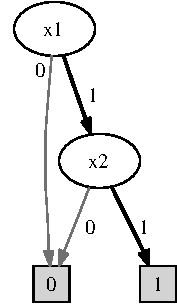
\includegraphics[%
    clip,
  scale=0.75]{obdd/figures/And1.pdf}&
&
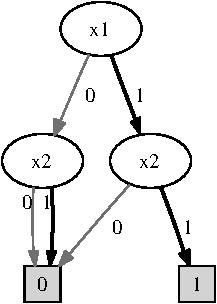
\includegraphics[%
  clip,
  scale=0.75]{obdd/figures/And1-full.pdf}\tabularnewline
Figure \ref{cap:BDDfill}(a)&
&
Figure \ref{cap:BDDfill}(b)\tabularnewline
\end{tabular}\end{center}
\caption{\label{cap:BDDfill}Adding dummy vertices}
\end{figure*}

One of the difficulties in developing and proving the protocol is
that OBDDs allow skipping of levels.  For example,
Figure~\ref{cap:BDDfill}(a) shows the OBDD for the Boolean function
$x_1 \wedge x_2$. Assume that the vertex at level $0$ is labeled with
$x_1$ and vertices at level $1$ are labeled with $x_2$. Suppose Alice
owns variable $x_1$ and Bob owns variable $x_2$. If Alice's input
is $1$, then Bob follows one more edge than if Alice's input were
$0$, which allows Bob to determine Alice's input. Compare this to
Figure~\ref{cap:BDDfill}(b), where a dummy vertex is added so
that, regardless of Alice's input, Bob has to follow the same number of
edges. In this case, Bob learns nothing about Alice's input. Before
Alice garbles the OBDDs, she adds dummy vertices so that each path
from the root to a terminal node has the same number of edges.  Alice adds
dummy nodes whenever $OBDD(f)$ allows Bob to skip levels when
evaluating the OBDD on his share of the input. Recall that the
$0$-successor and $1$-successor of $v$ is denoted by ${\it low}(v)$
and ${\it high}(v)$. For example, if node $n$ at level $j$ has node $n'''$ at level
$j+3$ as its $0$-successor, then Alice inserts two dummy nodes $n'$
and $n''$ at level $j+1$ and $j+2$ respectively. The $0$-successor of
node $n$ is changed to $n'$, both $0$ and $1$-successors of $n'$ are
set to $n''$, and both $0$ and $1$-successors of $n''$ are set to
$n'''$.


\begin{center}
\begin{boxfig*}{ht!}{
\textsc{\bf Input:} Both parties' inputs include the $OBDD(f)$ for the Boolean function
$f(x_1,x_2,\cdots,x_n)$ with the ordering $x_1 < x_2 < \cdots < x_n$.
Furthermore, Alice holds the inputs $(i_1,\ldots,i_k)$ corresponding
to the first $k$ variables $x_1,\ldots,x_k$, and Bob has the inputs
$(i_{k+1},\ldots,i_n)$. 
\vspace{1ex}
\begin{enumerate}
\item Alice performs the following steps:
\begin{enumerate}
\item She traverses the $OBDD(f)$ using her
input $(i_1,\cdots,i_k)$, which results in a node $v_{init}$ at level
$k$.

\item She uniformly and independently at random creates $(n-k)$ pairs
of secrets $(s_1^0,s_1^1),\cdots,(s_{n-k}^0,s_{n-k}^1)$.  In addition,
for each node $v$ in the $OBDD(f)$ whose level is between $k$ and $n-1$,
Alice also creates a secret $s_v$. 

\item She assigns a uniformly random label to each node whose level is
between $k$ and $n$. We refer to the randomly assigned label of node
$v$ using the notation $label(v)$.

\item Next, Alice augments $OBDD(f)$ with some number of dummy nodes
(to ensure that Bob always traverses $n-k$ nodes in his phase of the protocol). 


\item Alice garbles all nodes whose level is between $k$ and $n-1$
in the following manner. Let $v$ be a node in $OBDD(f)$ such $k \leq
{\it level}(v) \leq n-1$ and define ${\it level}(v)=\ell$. The encryption of node $v$, denoted
by $E^{(v)}$, is a label and a randomly ordered ciphertext pair
\[
\left(label(v)\,\,,\,\,E_{s_v \oplus s_{\ell-k+1}^0} (label(low(v)) \,\|\, s_{{\it low}(v)})\,\,\,,\,\,\,
E_{s_v \oplus s_{\ell-k+1}^1} (label(high(v)) \,\|\, s_{{\it high}(v)})\right)\,\,\,,
\]
where the labels are pre-pended to the secret with a separator symbol
and the order of the ciphertexts is determined by a fair coin
flip. Roughly speaking, the secrets corresponding to the $0$-successor
and $1$-successor of node $v$ are encrypted with the secret
corresponding to $v$ and its level.

Note that dummy nodes have the same structure as normal nodes, except
that the ciphertext pair contain encryptions of the same message since
dummy nodes have the same $0$ and $1$-successors. Provided the
encryption scheme is semantically secure, this poses no problem since
the keys are chosen uniformly at random.

Lastly, there are two terminal nodes of the form $(b,label(t_b))$ for
$b=0$ or $1$. Recall that $OBDD(f)$ has two terminal nodes, denoted as
$0$ and $1$, that are at level $n$.

\item Once Alice is done encrypting, she sends to Bob the encryption
of all nodes whose level is between $k$ and $n$ and the secret
$s_{v_{init}}$ corresponding to node $v_{init}$ at level $k$. We called
this the garbled OBDD.

\end{enumerate}

\item Bob performs the following steps:
\begin{enumerate}
\item He engages in $n-k$ 1-out-of-2 oblivious transfers to obtain the
secrets corresponding to his input. For example, if his input $i_j$ is
$0$, then he obtains the (level) secret $s_{j-k}^0$; otherwise, he
obtains the secret $s_{j-k}^1$.

\item Now Bob is ready to start his computation. Suppose
$i_{k+1}=0$. With $s_{1}^0$ and $s_{v_{init}}$, he decrypts both
ciphertexts in $E^{(v_{init})}$ and decides which gives the correct
result by using the verifiable range property of the encryption
scheme. Bob now has both $s_{{\it low}(v)}$ (the secret corresponding
to the $0$-successor of $v_{init}$) and $label(low(v))$ (which tells
Bob which encrypted node is used to evaluate his next
input). Continuing this way, Bob eventually obtains a label
corresponding to one of the terminal nodes, which determines the
result of the OBDD on the shared inputs. Bob sends this result to
Alice.
\end{enumerate}

\end{enumerate}
}
\vspace{-0.1cm}
\caption{\label{protbasicobdd} Protocol 1.}
\end{boxfig*}
\end{center}

We prove correctness and security in the case of semi-honest
parties. In the semi-honest model, both parties are assumed to perform
computations and send messages according to their prescribed actions
in the protocol. They may also record whatever they see during the
protocol (i.e. their own input and randomness, and the messages they
receive).  We refer readers to Goldreich's book~\cite{Goldreich:vol2}
for the complete definitions.  Claim~\ref{claim:protocol1correct}
proves that the protocol shown in Figure~\ref{protbasicobdd} is
correct; that is, Bob computes the function $f(i_1,\cdots,i_n)$.
Claim~\ref{claim:protocol1secure} proves that protocol 1 is secure
in the semi-honest model; that is, at the end of protocol 1, Alice only
knows its input and the value of the function $f(i_1,\cdots,i_n)$, and
similarly for Bob. For our proofs, we require the definition of elusive range and
efficiently verifiable range from Lindell and Pinkas~\cite{LP04}.
\begin{definition}
Let \alg{(G},\alg{E},\alg{D)} be a symmetric key encryption scheme
with key-generation, encryption, and decryption algorithms.
Denote the range of the scheme by
$\alg{Range}_n(k)=\{E_k(x)\}_{x\in\binset^n}$. We say that
\begin{enumerate}
	\item \alg{(G},\alg{E},\alg{D)} has an \textbf{elusive range}
	if for every probabilistic poly-time machine A, every
	polynomial $p(\cdot)$, and all sufficiently large $n$,
	$\Pr_{k\from\alg{G(1^n)}}[A(1^n)\in\alg{Range}_n(k)]<1/p(n)$.

	\item \alg{(G},\alg{E},\alg{D)} has an \textbf{efficiently
	verifiable range} if there exists a prob. poly-time
	machine $M$ such that $M(1^n,k,c)=1$ if and only if
	$c\in\alg{Range}_n(k)$.
\end{enumerate}
\end{definition}

\begin{claim} If the encryption scheme has an elusive range and the
oblivious transfer protocol is secure, then Protocol 1 is correct for
semi-honest Alice and Bob.
\label{claim:protocol1correct}
\end{claim}
\begin{proof}
First we show that every node in the garbled OBDD sent to Bob can be
evaluated correctly. For an encrypted node $v$, let $c_0$ and $c_1$ be
the first and second ciphertext term. Suppose $k$ is the key that Bob
obtains to decrypt the ciphertext in node $v$. Because the
encryption scheme is elusive and all the keys used in the garbled OBDD
are chosen uniformly and independently at random, it follows
immediately that, except with negligible probability, only one
ciphertext in an encrypted node decrypts correctly; that is,
either $c_0\in\alg{Range(k)}$ or $c_1\in\alg{Range(k)}$ but not
both. Hence, except with negligible probability, every node in the
garbled OBDD can be evaluated correctly.

By induction, we show that the correct key is obtained for every node
input and output. The base case is the key $s_{v_{init}}$ and the 
keys $s^{i_{k+1}}_{k+1},\ldots,s^{i_{n}}_{n}$ (corresponding to Bob's
input) obtained from Alice through the $n-k$ oblivious transfers. The
inductive step at node $v$ assumes that the correct label (pointing
Bob to node $v$) and node key $s_v$ was obtained in the previous
step. Furthermore, the correct level key $s_l^{i_l}$ was obtained by
executing an oblivious transfer protocol. Since every node in the
garbled OBDD can be evaluated correctly and the garbled OBDD is built by
a semi-honest Alice, Bob obtains the correct label and key output at
node $v$, which concludes the inductive step. We can conclude that the
entire garbled OBDD can be evaluated to give the correct result.\footnote{
Note that the negligible probability of error during
decryption can be removed by Alice first checking that every encrypted
node decrypts correctly before sending the garbled OBDD to Bob.
}
\end{proof}



\begin{claim} If the encryption scheme is semantically secure and has an
efficiently verifiable elusive range, and the oblivious transfer
protocol is secure, then Protocol 1 is secure against semi-honest
Alice and Bob.
\label{claim:protocol1secure}
\end{claim}
Proof of this claim is tedious and is given in Appendix~\ref{appendix:proof}.


\subsection{Protocol 2}
\label{subsec:protocol2}

The protocol presented in this section allows both Alice and Bob to
possess arbitrary input sets instead of assuming that Alice (and also
Bob) holds either the first $k$ or the last $n-k$ input variables.  In
this new protocol, before garbling the OBDD, Alice can reduce the size
of the OBDD by eliminating vertices whose labels correspond to Alice's
inputs.  Let $f(x_1,\cdots,x_n)$ be the function to be computed and
$X_A$ denotes the inputs of Alice. Alice first computes the OBDD  for the restriction $f
\mid_{X_A}$ of $f$ for the variables in its input
set $X_A$. Alice then encrypts the reduced OBDD and sends it to
Bob. During the restriction operation, all vertices whose labels
correspond to Bob's input should be included. If this is not the case,
then there is a risk that different restrictions could produce
different numbers of nodes, which would leak information to Bob about
Alice's inputs. For example, in Figure~\ref{cap:BDDpe}(a), where
Alice's value is $0$, there are only 2 nodes, but in
Figure~\ref{cap:BDDpe}(b), there are 3 nodes.
Figure~\ref{cap:BDDpe}(c) shows the result of retaining extra
vertices, in which case there are 4 nodes regardless of Alice's
inputs. The description of this protocol is given in
Figure~\ref{fig:protocol2}. The proof of correctness of this protocol
is almost identical to the one presented in
Section~\ref{sec:basicprotocol}. Example~\ref{example:protocol2} shows
an execution of this protocol on a small function.




\begin{figure*}

\begin{center}\begin{tabular}{cp{0.5in}p{1in}p{0.3in}c}
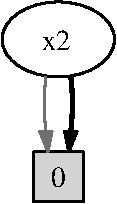
\includegraphics[%
  clip,
  scale=0.75]{obdd/figures/And1false.pdf}&
&
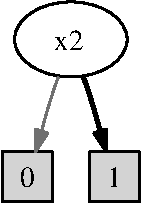
\includegraphics[%
  clip,
  scale=0.75]{obdd/figures/And1true.pdf}&
&
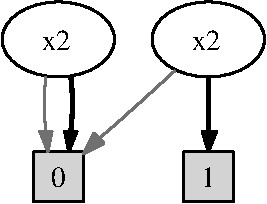
\includegraphics[%
  clip,
  scale=0.75]{obdd/figures/And1false2.pdf}\tabularnewline
Figure \ref{cap:BDDpe}(a)&
&
Figure \ref{cap:BDDpe}(b)&
&
Figure \ref{cap:BDDpe}(c)\tabularnewline
\end{tabular}\end{center}

\caption{\label{cap:BDDpe}OBDD restriction}

\end{figure*}

\begin{center}
\begin{boxfig}{ht!}{
\textsc{\bf Input:} Both parties' inputs include the $OBDD(f)$ for the Boolean function
$f(x_1,x_2,\cdots,x_n)$ with the ordering $x_1 < x_2 < \cdots < x_n$.
Furthermore, Alice holds the inputs for the variables in the set $X_A$ and
Bob holds the inputs for the variables in the set $X_B \; = \; \{ x_1,\cdots,x_n \} - X_A$.
\vspace{1ex}
\begin{enumerate}
\item Alice performs the following steps:
\begin{enumerate}
\item Alice computes the OBDD ${\cal O}_A$ for the function $f \mid_{X_A}$. This is the restriction
operation described in Section~\ref{sec:OBDDs}.

\item Alice encrypts the OBDD for the function $f \mid_{X_A}$ and sends it to Bob. This
step is exactly the same as for Protocol 1 described in Figure~\ref{protbasicobdd}. Alice also sends
the secret corresponding to the root of the OBDD ${\cal O}_A$. 


\end{enumerate}

\item The computation for Bob is exactly the same as that for Protocol 1. 

\end{enumerate}
}
\vspace{-0.1cm}
\caption{\label{fig:protocol2} Protocol 2.}
\end{boxfig}
\end{center}


\begin{example}
\label{example:protocol2}
\rm Assume that Alice and Bob want to compute $f(x_1,x_2)  \; = \; x_1 \wedge x_2$, where
Alice has input $x_1$ and Bob has input $x_2$, or in other words $X_A
\; = \; \{ x_1 \}$ and $X_B \; = \; \{ x_2 \}$.  Assume that $x_1 = 0$
and $x_2 = 1$. $OBDD(f)$ with dummy nodes is shown in
figure~\ref{cap:BDDfill}(b). Alice computes the OBDD for the function
$f \mid_{ x_1 \leftarrow 0}$, which results in a structure shown in
Figure~\ref{cap:BDDpe}(c).  Let the two nonterminal nodes in
Figure~\ref{cap:BDDpe}(c) be $v_1$ and $v_2$. First, Alice generates
$2$ secrets $s_{v_1}$ and  $s_{v_2}$, which are assigned
to the nodes $v_1$ and $v_2$, respectively.   Alice also
generates random labels for the four nodes in
Figure~\ref{cap:BDDpe}(c), and  generates a pair of secrets
$(s_1^0,s_1^1)$. The garbled OBDD corresponding to
Figure~\ref{cap:BDDpe}(c) is shown below (terminal nodes
are shown as $0$ and $1$ and lab denotes label). 
\begin{center}
\begin{tabular}{|l|} \hline
$(lab(v_1), E_{s_{v_1} \oplus s_1^0} (lab(0)  \,\|\, s_0), E_{s_{v_1} \oplus s_1^1} (lab(0) \,\|\, s_0))$ \\ \hline
$(lab(v_2), E_{s_{v_2} \oplus s_1^0} (lab(0) \,\|\, s_0), E_{s_{v_2} \oplus s_1^1} (lab(1) \,\|\, s_1))$ \\ \hline
$(0,lab(0))$ \\ \hline
$(1,lab(1))$ \\ \hline
\end{tabular}
\end{center}
Alice reveals the secret $s_{v_1}$ corresponding node $v_1$.
Alice and Bob engage in a 1-out-of-2 ($OT^2_1$) protocol and Bob obtains the secret $s_1^1$ (recall that
$x_2 = 1$).
Bob can now decrypt the second component of the first entry of the garbled OBDD and
obtain $label(0) \,\|\, s_0$, and  Bob can infer that the output is $0$.
\end{example}

\begin{claim} If the encryption scheme has an elusive range and the
oblivious transfer protocol is secure, then Protocol 2 is correct for
semi-honest Alice and Bob.
\label{claim:protocol2correct}
\end{claim}
\begin{proof}
The proof of this claim is exactly same as the proof of Claim~\ref{claim:protocol1correct}.
One has to assume that the restriction operation used by Alice is correct.
\end{proof}

\begin{claim} If the encryption scheme is semantically secure and has an
efficiently verifiable elusive range, and the oblivious transfer
protocol is secure, then Protocol 2 is secure against semi-honest
Alice and Bob.
\label{claim:protocol2secure}
\end{claim}
Proof of this claim is tedious and is given in Appendix~\ref{appendix:proof}.
